% This LaTeX was auto-generated from MATLAB code.
% To make changes, update the MATLAB code and export to LaTeX again.

\documentclass{article}

\usepackage[utf8]{inputenc}
\usepackage[T1]{fontenc}
\usepackage{lmodern}
\usepackage{graphicx}
\usepackage{color}
\usepackage{hyperref}
\usepackage{amsmath}
\usepackage{amsfonts}
\usepackage{epstopdf}
\usepackage[table]{xcolor}
\usepackage{matlab}

\sloppy
\epstopdfsetup{outdir=./}
\graphicspath{ {./Lab07_images/} }

\begin{document}

\matlabtitle{LAB 7: STATE-SPACE DESIGN FOR POSITION CONTROL IN A DC MOTOR}

\begin{matlabcode}
%---------------------------------------
% Fill in your student Name and ID.
Students.Name = 'Seyed Yazdan Zinati';
Students.ID = '260928077';
%---------------------------------------
\end{matlabcode}


\matlabheading{\textbf{0. Objectives}}

\begin{par}
\begin{flushleft}
In this lab, we will experiment with different controller design to regulate the angular position of a DC Motor. For this we will use state-space representation in \texttt{\textbf{MATLAB}} and the function \textbf{lsim} to simulate the response of continuous linear systems to arbitrary inputs.
\end{flushleft}
\end{par}

\begin{par}
\begin{flushleft}
In section 1, we will define the DC Motor model. In section 2, we will design an output feedback controller for angular position control. In section 3, we will study the effect of model mismatch on the output feedback control. Finally, in section 4, we will design a state feedback with an integral component to reduce the disturbance effects.
\end{flushleft}
\end{par}

\matlabheading{\textbf{1. State-Space Representation of a DC Motor}}

\begin{par}
\begin{flushleft}
A DC motor can be characterized by the following parameters:
\end{flushleft}
\end{par}

\begin{matlabcode}
param.Kt = 0.035; % Torque proportionality constant (Kg m2 /s2/A) (N.m/A)
param.Ke = 0.035; % Back electromotive proportionality constant (V/rad/s)
param.L = 5e-3; % Electric inductance (H)
param.R = 0.1; % Terminal resistance (Ohm)
param.J = 5e-4; % Rotor moment of inertia (kg.m2)
param.b = 1e-06; % Rotor viscous friction constant (Kg.m2/s) (N.m.s)
\end{matlabcode}


\begin{par}
\begin{flushleft}
Notice that these parameters differ from the one used for the hardware Qnet DC Motor, and are chosen for the purpose of this lab experiments. The complete state of the DC Motor is represented by $x(t)$
\end{flushleft}
\end{par}

\begin{par}
$$x(t)=\left(\begin{array}{c}
\theta (t)\\
\omega (t)\\
i(t)
\end{array}\right)$$
\end{par}

\begin{par}
\begin{flushleft}
where $\theta (t)$ is the angular position of the rotor, $\omega (t)$ is the angular velocity, and $i(t)$ is the current. The state-space representation of the DC Motor can be written as.
\end{flushleft}
\end{par}

\begin{par}
$${{\frac{d}{dt}x(t)=\left(\begin{array}{ccc}
0 & 1 & 0\\
0 & -{{\frac{b}{J}}} & {{\frac{K_t }{J}}}\\
0 & -{{\frac{K_e }{L}}} & -{{\frac{R}{L}}}
\end{array}\right)x(t)+\left(\begin{array}{c}
0\\
0\\
{{\frac{1}{L}}}
\end{array}\right)v(t)}}$$
\end{par}

\begin{par}
\begin{flushleft}
We are interested on controlling the angular position $\theta (t)=\left(\begin{array}{ccc}
1 & 0 & 0
\end{array}\right)x(t)$ to track a step input of 90 degrees.
\end{flushleft}
\end{par}

\begin{par}
\begin{flushleft}
The state-space representation of the DC Motor can be written as.
\end{flushleft}
\end{par}

\begin{matlabcode}
A = [ ...
    0, 1, 0; ...
    0, -param.b / param.J, param.Kt / param.J; ...
    0, -param.Ke / param.L, -param.R / param.L];
B = [ ...
    0; ...
    0; ...
    1 / param.L];
C = [1, 0, 0];
D = 0;
\end{matlabcode}


\matlabheading{\textbf{2. Position Control with Output Feedback}}

\matlabheading{\textit{2.1 Full state feedback}}

\begin{par}
\begin{flushleft}
In this section we assume that the state $x(t)$ is available at any time. Thus, we will design a state feedback controller of the form:
\end{flushleft}
\end{par}

\begin{par}
$$v(t)=-Kx(t)+Nr(t)$$
\end{par}

\begin{par}
\begin{flushleft}
\textless{}\textless{}fig\_lab07\_full\_state\_feedback.png\textgreater{}\textgreater{}
\end{flushleft}
\end{par}

\matlabheading{\textit{Question 1 (0.5 marks)}}

\begin{par}
\begin{flushleft}
Is the system controllable in the proposed state representation?
\end{flushleft}
\end{par}

\begin{matlabcode}
G = ss(A, B, C, D);
Gs = tf(G);


controllabilityMatrix = ctrb(A, B)
\end{matlabcode}
\begin{matlaboutput}
controllabilityMatrix = 3x3    
1.0e+05 *

         0         0    0.1400
         0    0.1400   -2.8003
    0.0020   -0.0400   -0.1800

\end{matlaboutput}
\begin{matlabcode}

if det(controllabilityMatrix) ~= 0
    disp('The system is controllable')
else
    disp('The system is not controllable')
end
\end{matlabcode}
\begin{matlaboutput}
The system is controllable
\end{matlaboutput}


\matlabheading{\textit{Question 2 (2 marks)}}

\begin{enumerate}
\setlength{\itemsep}{-1ex}
   \item{\begin{flushleft} Design the feedback gain K such that the state feedback places the closed-loop poles at the following locations: $-15\pm 15j$, and -150. \end{flushleft}}
   \item{\begin{flushleft} Find the value of the pre-compensator N that will make the steady state error 0. \end{flushleft}}
   \item{\begin{flushleft} Complete the code to test the designed state-feedback controller. \end{flushleft}}
\end{enumerate}

\begin{matlabcode}
p1 = -15 + 15j;
p2 = -15 - 15j; 
p3 = -150; 

Kpoles = [p1, p2, p3]
\end{matlabcode}
\begin{matlaboutput}
Kpoles = 1x3 complex    
1.0e+02 *

  -0.1500 + 0.1500i  -0.1500 - 0.1500i  -1.5000 + 0.0000i

\end{matlaboutput}
\begin{matlabcode}

K = place(A, B, Kpoles)
\end{matlabcode}
\begin{matlaboutput}
K = 1x3    
    4.8214    0.3185    0.8000

\end{matlaboutput}


\begin{matlabcode}
A1 = A - B * K;
Gc1 = ss(A1, B, C, D);
dcGainCL = dcgain(tf(Gc1));

N = 1/dcGainCL 
\end{matlabcode}
\begin{matlaboutput}
N = 4.8214
\end{matlaboutput}


\begin{matlabcode}
dt = 1e-3; % sampling time
t = 0:dt:2; % time signal
r = 90 * pi / 180 * ones(size(t)); % reference signal


Hcl = Gc1;


w = lsim(Hcl, N*r, t)'; % simulate the output
v = -K * lsim(ss(Hcl.A, Hcl.B, eye(3), 0), N*r, t)' + N * r; % simulate the command

customStep(sprintf('Full State Feedback'), t, w, r, v)
\end{matlabcode}
\begin{center}
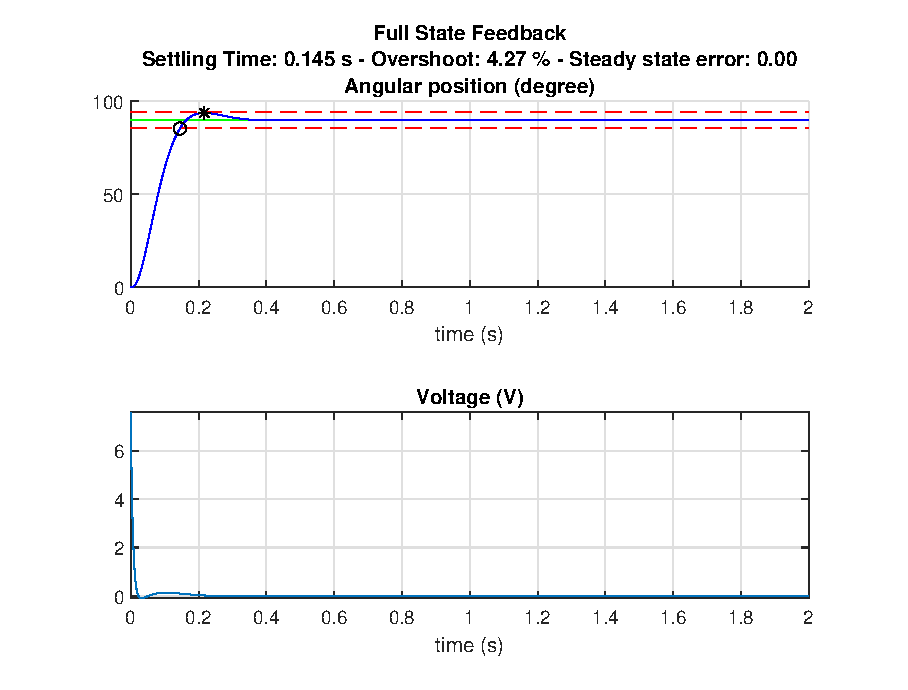
\includegraphics[width=\maxwidth{56.196688409433015em}]{figure_0.eps}
\end{center}


\matlabheading{\textit{2.2 Output feedback with state observer}}

\begin{par}
\begin{flushleft}
We assume that the state can't be fully measured and only the angular position can be measured. We will design a Luenberger observer based on the known model and the output $\theta (t)$. Recall that the equations of Luenberger observer are:
\end{flushleft}
\end{par}

\begin{par}
$${{\frac{d}{dt}\hat{x} (t)=A\hat{x} (t)+Bv(t)+L(Cx(t)-C\hat{x} (t))}}$$
\end{par}

\begin{par}
\begin{flushleft}
where $L$ is the Luenberger gain.
\end{flushleft}
\end{par}

\begin{par}
\begin{flushleft}
\textless{}\textless{}fig\_lab07\_output\_feedback.png\textgreater{}\textgreater{}
\end{flushleft}
\end{par}

\matlabheading{\textit{Question 3 (0.5 marks)}}

\begin{par}
\begin{flushleft}
Is the system observable in the proposed state representation?
\end{flushleft}
\end{par}

\begin{matlabcode}
observabilityMatrix = obsv(A, C);


if det(observabilityMatrix) ~= 0
    disp('The system is observable')
else
    disp('The system is not observable')
end
\end{matlabcode}
\begin{matlaboutput}
The system is observable
\end{matlaboutput}
\begin{matlabcode}

\end{matlabcode}


\matlabheading{\textit{Question 4 (1 marks)}}

\begin{par}
\begin{flushleft}
Design a Luenberger state estimator such that the eigenvalues of the observer are $-10\pm 10j$, and -100.
\end{flushleft}
\end{par}

\begin{matlabcode}
Lpoles = [-10+10j, -10-10j, -100];

L = place(A', C', Lpoles)'
\end{matlabcode}
\begin{matlaboutput}
L = 3x1    
   99.9980
 -290.2000
 -331.4146

\end{matlaboutput}


\begin{par}
\begin{flushleft}
The state space representation of the output feedback system with a state observer can be represented by the augmented state:
\end{flushleft}
\end{par}

\begin{par}
$$x_{aug} (t)=\left(\begin{array}{c}
x(t)\\
\hat{x} (t)
\end{array}\right)$$
\end{par}

\begin{par}
\begin{flushleft}
and the feedback law is:
\end{flushleft}
\end{par}

\begin{par}
$$v(t)=-K\hat{x} (t)+Nr$$
\end{par}

\begin{par}
\begin{flushleft}
With these notations, we can write the augmented state space equations as a function of A, B, C, K, and L
\end{flushleft}
\end{par}

\begin{par}
$${{\frac{d}{dt}x_{aug} (t)=\left(\begin{array}{cc}
A & -BK\\
LC & A-LC-BK
\end{array}\right)x_{aug} (t)+\left(\begin{array}{c}
B\\
B
\end{array}\right)v(t)}}$$
\end{par}

\matlabheading{\textit{Question 5 (1.5 marks)}}

\begin{enumerate}
\setlength{\itemsep}{-1ex}
   \item{\begin{flushleft} Write the augmented state-space representation matrices $A_{aug}$ and $B_{aug}$. \end{flushleft}}
   \item{\begin{flushleft} Complete the code to simulate the response of output feedback system to follow a step input (use the same feedback gain $N$, and $K$ from section 1.1). \end{flushleft}}
\end{enumerate}

\begin{matlabcode}
% 1 -

Aaug = [A, -B*K; L*C, A-L*C-B*K];

Baug = [B; B];


% 2 -
Caug = [1, 0, 0, 0, 0, 0];

 
% define the augmented closed loop system
Hcl = ss(Aaug, Baug, Caug, 0);

% simulate the output
w = lsim(Hcl, N*r, t)';

w = w(:)'; % make the output a row array
v = -K * lsim(ss(Hcl.A, Hcl.B, [zeros(3), eye(3)], 0), N*r, t)' + N * r; % simulate the command

customStep(sprintf('Output Feedback'), t, w, r, v)
\end{matlabcode}
\begin{center}
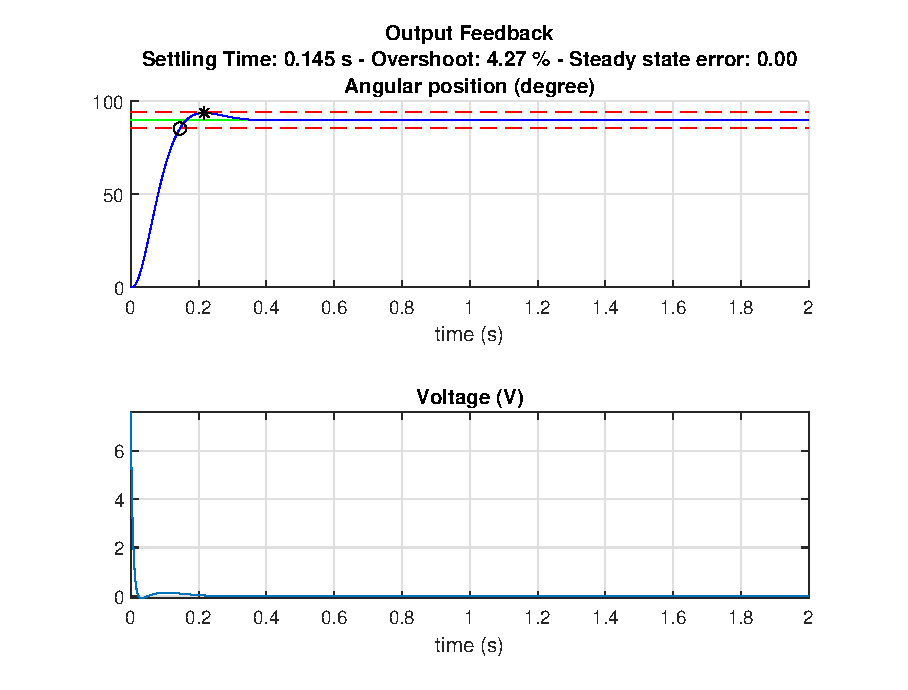
\includegraphics[width=\maxwidth{56.196688409433015em}]{figure_1.eps}
\end{center}


\matlabheading{\textit{Question 6 (1 marks)}}

\begin{par}
\begin{flushleft}
Let's change the Luenberger gain such as the observer dynamic is 10 times slower. re-run the experiment. What do you observe? Justify your answer.
\end{flushleft}
\end{par}

\begin{matlabcode}
Lnewpoles = 0.1 * Lpoles;

Lnew = place(A', C', Lnewpoles)';

K = place(A, B, Kpoles);

Aaug = [A, -B*K; Lnew*C, A-Lnew*C-B*K];

Baug = [B; B];

Caug = [1, 0, 0, 0, 0, 0];

% define the closed loop system
Hcl = ss(Aaug, Baug, Caug, 0);

% simulate the output
w = lsim(Hcl, N*r, t)';


w = w(:)'; % make the output a row array
v = -K * lsim(ss(Hcl.A, Hcl.B, [zeros(3), eye(3)], 0), N*r, t)' + N * r; % simulate the command

customStep(sprintf('Output Feedback with smaller gain'), t, w, r, v)
\end{matlabcode}
\begin{center}
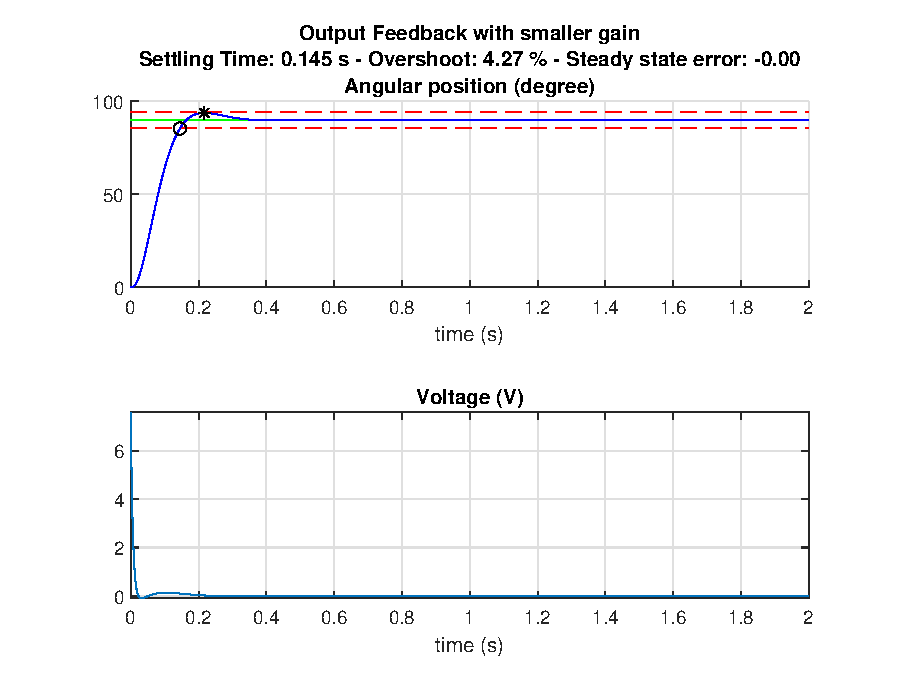
\includegraphics[width=\maxwidth{56.196688409433015em}]{figure_2.eps}
\end{center}


\begin{matlabcode}
% We can observe that all the graphs in question 2, 5, and 6
% are the same. They have the same settling time of 0.145s, 
% OS = 4.27% and a steady state error of 0. The angular position
% is also stable and constant at the end. 

% We can see that the observer being faster or slower (by changing L)
% doesn't affect the output feedback of the system
\end{matlabcode}


\matlabheading{\textbf{3. Effects of wrong model}}

\begin{par}
\begin{flushleft}
As seen in section 2 the importance of the Luenberger estimator will only be visible in case the dynamics of the model are not completely known. For example, in this section we assume that in the real DC Motor the inertia is 3 times what we initially thought. Which means that the true dynamics of the DC Motor are:
\end{flushleft}
\end{par}

\begin{par}
\begin{flushleft}
\textless{}\textless{}fig\_lab07\_estimator\_wrong\_model.png\textgreater{}\textgreater{}
\end{flushleft}
\end{par}

\begin{matlabcode}
Jreal = 3 * param.J;

Areal = [ ...
    0, 1, 0; ...
    0, -param.b / Jreal, param.Kt / Jreal; ...
    0, -param.Ke / param.L, -param.R / param.L];
\end{matlabcode}


\begin{par}
\begin{flushleft}
For the purpose of this experiment we assume that we don't know about the true $A_{real}$ and we only use $A$ in the estimator dynamics.
\end{flushleft}
\end{par}

\matlabheading{\textit{Question 7 (1.5 marks)}}

\begin{enumerate}
\setlength{\itemsep}{-1ex}
   \item{\begin{flushleft} Re-run the experiment using the same gains $N$, $K$, and $L$. But this time replace the transition matrix of the state space model of the DC Motor by $A_{real}$. What do you observe? \end{flushleft}}
   \item{\begin{flushleft} Change the design of $L$ such as the observer is 5 times faster. What do you observe? \end{flushleft}}
\end{enumerate}

\begin{matlabcode}
% 1
Aaug = [Areal, -B*K; L*C, Areal-L*C-B*K];

Baug = [B; B];

Caug = [1, 0, 0, 0, 0, 0];

% define the closed loop system
Hcl = ss(Aaug, Baug, Caug, 0);

% simulate the output
w = lsim(Hcl, N*r, t)';


w = w(:)'; % make the output a row array
v = -K * lsim(ss(Hcl.A, Hcl.B, [zeros(3), eye(3)], 0), N*r, t)' + N * r; % simulate the command

customStep(sprintf('Output Feedback with wrong model'), t, w, r, v)
\end{matlabcode}
\begin{center}
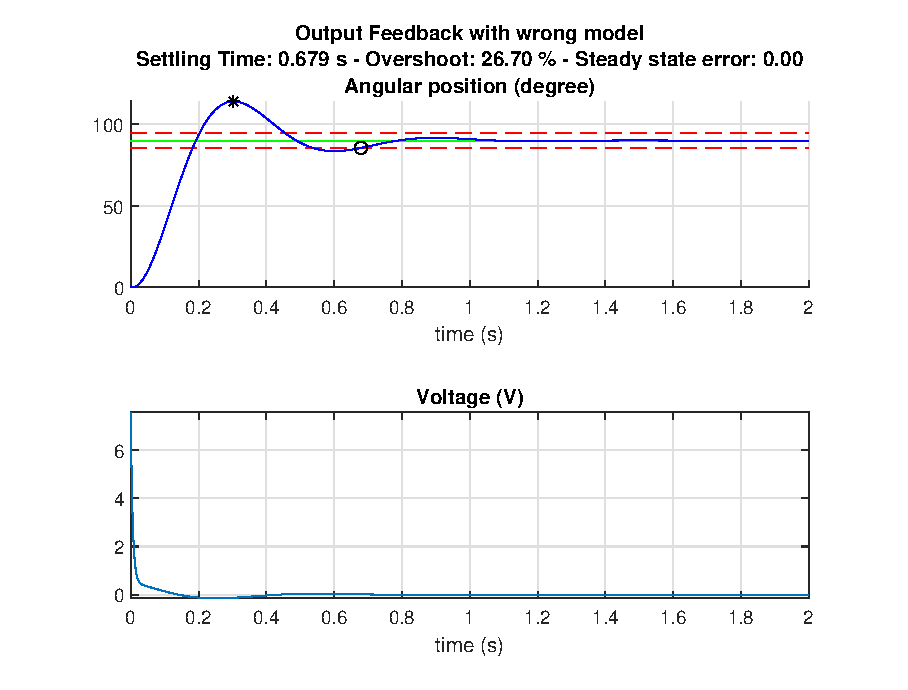
\includegraphics[width=\maxwidth{56.196688409433015em}]{figure_3.eps}
\end{center}


\begin{matlabcode}
% We can observe a higher overshoot percentage (26.70% vs 4.27%) and we can 
% also see that the settling time has increased. We can thus say
% that with higher inertia comes higher overshoot and larger settling time. 
\end{matlabcode}


\begin{matlabcode}
% 2 -

Lnewpoles = 5 * Lpoles;

Lnew = place(A', C', Lnewpoles)';

K = place(A, B, Kpoles);

Aaug = [Areal, -B*K; Lnew*C, Areal-Lnew*C-B*K];

Baug =  [B;B];

Caug = [1, 0, 0, 0, 0, 0];

% define the closed loop system
Hcl = ss(Aaug, Baug, Caug, 0); 

% simulate the output
w = lsim(Hcl, N*r, t)';


w = w(:)'; % make the output a row array
v = -K * lsim(ss(Hcl.A, Hcl.B, [zeros(3), eye(3)], 0), N*r, t)' + N * r; % simulate the command

customStep(sprintf('Output Feedback with wrong model and tuning'), t, w, r, v)
\end{matlabcode}
\begin{center}
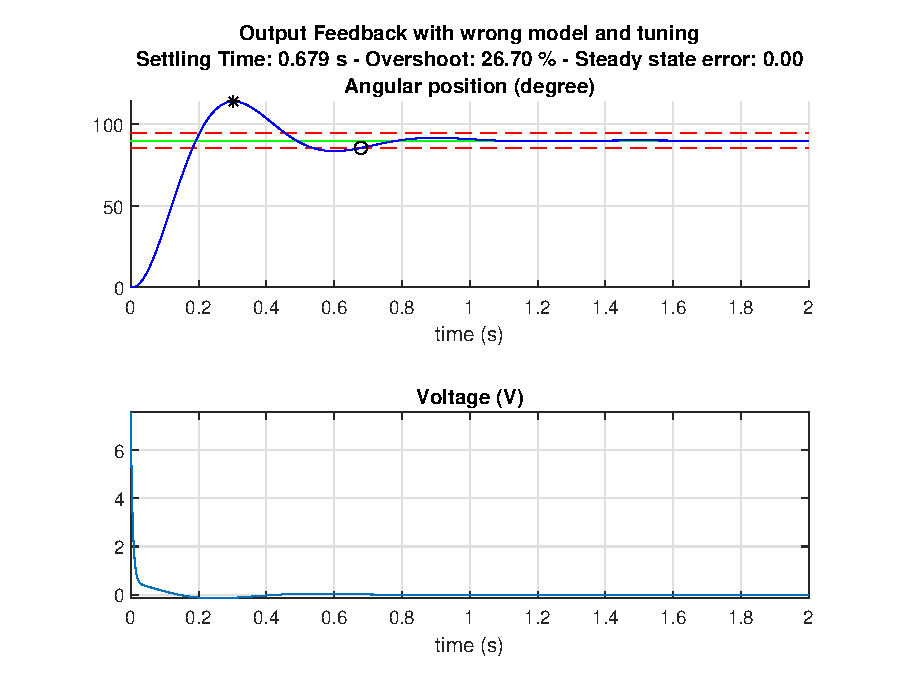
\includegraphics[width=\maxwidth{56.196688409433015em}]{figure_4.eps}
\end{center}


\begin{matlabcode}
% The observer being faster or slower (by changing L)
% doesn't affect the output feedback of the system
\end{matlabcode}


\matlabheading{\textbf{4. Disturbance and Integral Design}}

\matlabheading{\textit{4.1 Experiment with an additive disturbance}}

\begin{par}
\begin{flushleft}
In this section we want to study the effects of a voltage disturbance on the state feedback controller. For this, we will simulate the effects of an additive disturbance into the voltage command of value $d=4V$ at time = 1s.
\end{flushleft}
\end{par}

\begin{par}
\begin{flushleft}
To simplify the problem, we will consider that the whole state is available, that we know the exact model of the DC Motor (same in section 1), and that we have designed a full feedback controller $K$, and $N$.
\end{flushleft}
\end{par}

\matlabheading{Question 8 (0 marks)}

\begin{par}
\begin{flushleft}
What do you expect to happen to the angular position of the DC motor after applying a voltage command $d=4V$ at time = 1s?
\end{flushleft}
\end{par}

\begin{matlabcode}
% There will be the superposition of another response starting at 1s
% So the angular position should increase to a higher value and
% settle eventually with a higher the steady state error.
\end{matlabcode}


\begin{par}
\begin{flushleft}
Let's simulate the result of adding such a disturbance in the closed-loop system
\end{flushleft}
\end{par}

\begin{matlabcode}
K = place(A, B, Kpoles);

d = zeros(size(t));
d(t >= 1) = 4; % disturbance signal

Hcl = ss(A-B*K, B, C, 0); % define the closed loop system
w = lsim(Hcl, N*r+d, t)'; % simulate the output
v = -K * lsim(ss(Hcl.A, Hcl.B, eye(3), 0), N*r+d, t)' + N * r + d; % simulate the command

customStep(sprintf('State Feedback with disturbance'), t, w, r, v)
\end{matlabcode}
\begin{center}
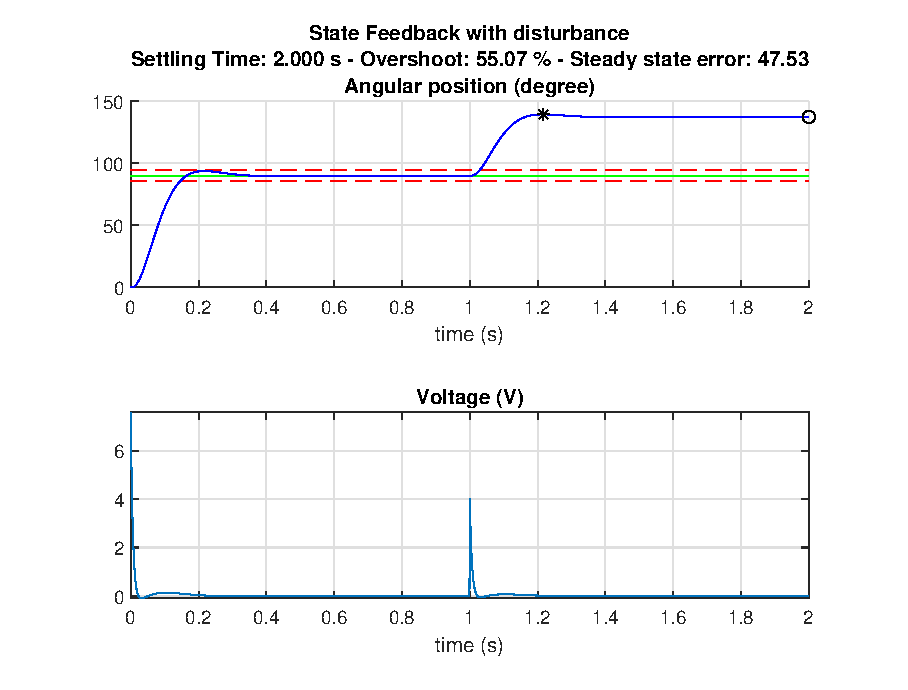
\includegraphics[width=\maxwidth{56.196688409433015em}]{figure_5.eps}
\end{center}


\matlabheading{Question 9 (0.5 marks)}

\begin{par}
\begin{flushleft}
What is the steady state error? What is the closed-loop system type?
\end{flushleft}
\end{par}

\begin{matlabcode}
% ss error 
steadyStateError = 47.53
\end{matlabcode}
\begin{matlaboutput}
steadyStateError = 47.5300
\end{matlaboutput}
\begin{matlabcode}

% Because the steady state error is a non zero constant with step input, 
% our closed loop system can be identified as TYPE0. 
\end{matlabcode}


\matlabheading{\textit{4.2 state feedback with integral term}}

\begin{par}
\begin{flushleft}
We can add an integral term to the feedback controller to increase the type of the system. The integral equation is
\end{flushleft}
\end{par}

\begin{par}
$$x_n (t)=r(t)-Cx(t)$$
\end{par}

\begin{par}
\begin{flushleft}
The augmented system is
\end{flushleft}
\end{par}

\begin{par}
$$x_{aug} (t)=\left(\begin{array}{c}
x(t)\\
x_n (t)
\end{array}\right)$$
\end{par}

\begin{par}
\begin{flushleft}
and the feedback law is:
\end{flushleft}
\end{par}

\begin{par}
$$v(t)=-Kx(t)+K_e x_n (t)$$
\end{par}

\begin{par}
\begin{flushleft}
The equivalent system can be seen as a closed-loop system where the open-loop dynamics is defined by
\end{flushleft}
\end{par}

\begin{par}
$$\tilde{A} =\left(\begin{array}{cc}
A & 0\\
-C & 0
\end{array}\right)$$
\end{par}

\begin{par}
$$\tilde{B} =\left(\begin{array}{c}
B\\
0
\end{array}\right)$$
\end{par}

\begin{par}
\begin{flushleft}
and a unity feedback
\end{flushleft}
\end{par}

\begin{par}
$$v(t)=-\left(\begin{array}{cc}
K & -K_e 
\end{array}\right)x_{aug} (t)$$
\end{par}

\matlabheading{Question 10 (1.5 marks)}

\begin{enumerate}
\setlength{\itemsep}{-1ex}
   \item{\begin{flushleft} Design $K$ and $Ke$ such as the poles of the feedback system are: $-15\pm 15j$, and $-150\pm 150j$. \end{flushleft}}
   \item{\begin{flushleft} Complete the code to run the simulation. \end{flushleft}}
   \item{\begin{flushleft} What do you observe? \end{flushleft}}
\end{enumerate}

\begin{matlabcode}
% 1 - use place in the augmented closed-loop with integral system
p1d = -15 + 15i;
p2d = -15 - 15i;
p3d = -150 * (1 + 1i);
p4d = -150 * (1 - 1i);

Atilde = [A, zeros(3, 1); -C, 0];
Btilde = [B; 0];
Kall = place(Atilde, Btilde, [p1d, p2d, p3d, p4d])
\end{matlabcode}
\begin{matlaboutput}
Kall = 1x4    
1.0e+03 *

    0.1061    0.0039    0.0015   -1.4464

\end{matlaboutput}
\begin{matlabcode}
K = Kall(1, 1:3) % Gain of the 1st 3 states 
\end{matlabcode}
\begin{matlaboutput}
K = 1x3    
  106.0714    3.8542    1.5500

\end{matlaboutput}
\begin{matlabcode}
Ke = -Kall(1, 4) % The gain not associated with first 3 states 
\end{matlabcode}
\begin{matlaboutput}
Ke = 1.4464e+03
\end{matlaboutput}


\begin{matlabcode}
% 2 - Run the experiment

d = zeros(size(t));
d(t >= 1) = 4; % disturbance signal

% define the augmented closed-loop system

AtildeCl = Atilde - Btilde * Kall
\end{matlabcode}
\begin{matlaboutput}
AtildeCl = 4x4    
1.0e+05 *

         0    0.0000         0         0
         0   -0.0000    0.0007         0
   -0.2121   -0.0078   -0.0033    2.8929
   -0.0000         0         0         0

\end{matlaboutput}
\begin{matlabcode}


% simulate the output
yr = lsim(ss(AtildeCl, [0; 0; 0; 1], [1, 0, 0, 0], 0), r, t)'; %response to reference
yd = lsim(ss(AtildeCl, Btilde, [1, 0, 0, 0], 0), d, t)'; %response to disturbance
w = yr + yd;

v = -[K, -Ke] * lsim(ss(AtildeCl, [[0; 0; 0; 1], Btilde], eye(4), 0), [r; d], t)' + d; % simulate the command

customStep(sprintf('Integral State Feedback with disturbance'), t, w, r, v)
\end{matlabcode}
\begin{center}
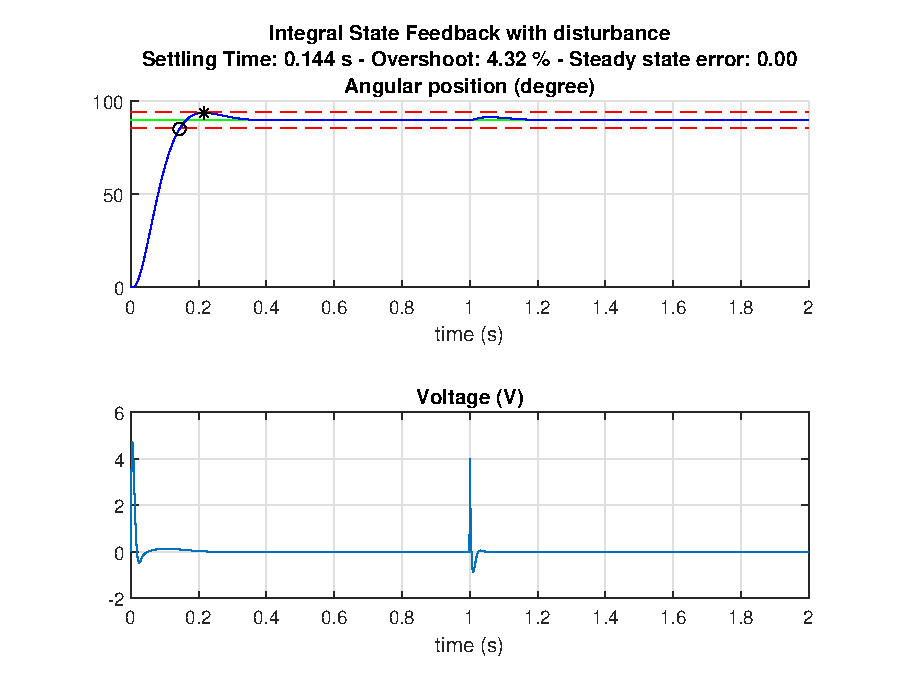
\includegraphics[width=\maxwidth{56.196688409433015em}]{figure_6.eps}
\end{center}


\begin{matlabcode}
% 3 - 
% The same 4V disturbance slightly changes the angular position, 
% which quickly returns to the original steady-state value without the same
% "permanent" gain as before
\end{matlabcode}


\matlabheading{\textbf{5. Useful Functions}}

\matlabheading{\textit{5.1 Custom step response}}

\begin{matlabcode}
function customStep(figTitle, t, w, r, v)
% calculate response characteristics and plot results
settlingTimeIdx = find(round((w - 0.95 * r)*180/pi, 1) <= 0.05 | round((w - 1.05 * r)*180/pi, 2) >= -0.05, 1, 'last');
[~, overshootIdx] = max(w);
steadyStateError = (180 / pi) * (w(end) - r(end));

figure;
clf;
hold on;
subplot(2, 1, 1)
hold on;
plot(t, (180 / pi)*0.95*r, '--r');
plot(t, (180 / pi)*1.05*r, '--r');
plot(t, (180 / pi)*r, 'g');
plot(t, (180 / pi)*w, 'b');
plot(t(settlingTimeIdx), (180 / pi)*w(settlingTimeIdx), 'ok')
plot(t(overshootIdx), (180 / pi)*w(overshootIdx), '*k')
grid on;
title(sprintf(['%s\n', ...
    'Settling Time: %4.3f s - Overshoot: %03.2f %% - Steady state error: %3.2f\n', ...
    'Angular position (degree)'], ...
    figTitle, ...
    t(settlingTimeIdx), ...
    100*(w(overshootIdx) - r(end))/r(end), ...
    steadyStateError))
xlabel('time (s)')
subplot(2, 1, 2)
plot(t, v);
grid on;
title('Voltage (V)');
xlabel('time (s)')
drawnow;
end
\end{matlabcode}

\end{document}
